%!TEX TS-program=xelatex
%!USE flag=shell-escape
\documentclass{beamer}
\usepackage{HSE-theme/beamerthemeHSE} % Подгружаем тему

%%% Работа с русским языком и шрифтами
\usepackage[english,russian]{babel}   % загружает пакет многоязыковой вёрстки
\usepackage{fontspec}      % подготавливает загрузку шрифтов Open Type, True Type и др.
\defaultfontfeatures{Ligatures={TeX},Renderer=Basic}  % свойства шрифтов по умолчанию
\setmainfont[Ligatures={TeX,Historic}]{Myriad Pro} %  установите шрифты Myriad Pro или (при невозможности) замените здесь на другой шрифт, который есть в системе — например, Arial
\setsansfont{Myriad Pro}  %  установите шрифты Myriad Pro или (при невозможности) замените здесь на другой шрифт, который есть в системе — например, Arial
\setmonofont{Courier New}
\uselanguage{russian}
\languagepath{russian}
\deftranslation[to=russian]{Theorem}{Теорема}
\deftranslation[to=russian]{Definition}{Определение}
\deftranslation[to=russian]{Definitions}{Определения}
\deftranslation[to=russian]{Corollary}{Следствие}
\deftranslation[to=russian]{Fact}{Факт}
\deftranslation[to=russian]{Example}{Пример}
\deftranslation[to=russian]{Examples}{Примеры}

\usepackage{multicol} 		% Несколько колонок
\graphicspath{{images/}}  	% Папка с картинками

% \usepackage[backend=biber]{biblatex}
% \addbibresource{used_sources.bib}
\usepackage{caption}
\newlength{\mylen}


%%% Информация об авторе и выступлении
\title[Заголовок]{\footnotesize Факультет Компьютерных Наук\\Департамент
Программной Инженерии\\Выпускная квалификационная работа}
\subtitle{Криптографические алгоритмы и протоколы для распределенных реестров\\
Cryptographic Algorithms and Protocols for Distributed Ledgers}
\author[Куприянов К.И.]{\scriptsize Выполнил: студент
гр.БПИ151 Куприянов Кирилл\\Научный руководитель: Профессор, руководитель ДПИ,\\к.т.н. Авдошин Сергей Михайлович}
\institute[Высшая школа экономики]{}
\date{\the\year}

\begin{document}	% Начало презентации
\frame[plain]{
    \maketitle
}

% \frame[plain]{\titlepage}	% Титульный слайд

% \section{Просто слайд с текстом}
% \subsection{Просто слайд с текстом}

\begin{frame}
\frametitle{Предметная область}
	\begin{multicols}{2}
        1. Распределённые реестры -- база данных, которая распределена между
        несколькими сетевыми узлами или вычислительными устройствами. Каждый
        узел получает данные из других узлов и хранит полную копию реестра.
        Обновления узлов происходят независимо друг от друга

		\columnbreak

        2. Криптография -- наука, изучающая математические методы защиты
        информации, методы преобразования, обеспечивающие ее конфиденциальность
        и аутентичность.\\
        \emph{Разделы: асимметричные криптосистемы, системы электронной цифровой
        подписи (ЭЦП), хеш-функции}
		\medskip
		% \includegraphics[width=\columnwidth]{skidka.png}
	\end{multicols}
\end{frame}

\begin{frame}
\frametitle{Определения}
        \begin{itemize}
            \item Симметричное шифрование --- для шифрования и расшифровывания
                  применяется один и тот же криптографический ключ
            \item Асимметричное шифрование --- открытый ключ передаётся по
                  открытому каналу и используется для проверки ЭП и для
                  шифрования сообщения
            \item Электронная подпись (ЭП) --- электронный документ, полученный
                  преобразованием закрытым ключом подписи. Позволяет проверить
                  \emph{целостность, авторство и неотказуемость}
        \end{itemize}
\end{frame}

\begin{frame}[c]
    \frametitle{Обоснование актуальности работы}
    \framesubtitle{Популярность скидок в интернете}

    \begin{multicols}{2}
    \begin{figure}
        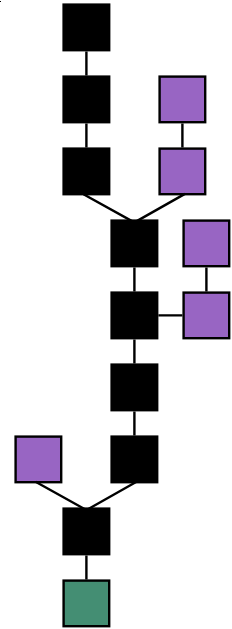
\includegraphics[height=0.8\columnwidth]{blockchain.png}
        \captionsetup{labelformat=empty}
        \caption{Блокчейн}
    \end{figure}

        \columnbreak

        \begin{figure}
            
\includegraphics[height=0.8\columnwidth]{ton.png}
            \captionsetup{labelformat=empty}
            \caption{Криптовалюты}
        \end{figure}
    \end{multicols}
\end{frame}

\begin{frame}
    \frametitle{Цель и задачи работы}
    \textbf{Цель}: Анализ и классификация актуальных криптографических
    алгоритмов для распределённых реестров в мире.\\
    \textbf{Задачи}:
    \begin{itemize}
        \item Выявить популярные распределённые реестры; выделить и изучить
              криптографические алгоритмы в них
        \item Замерить параметры алгоритмов
        \item Классифицировать их по:
        \begin{itemize}
            \item Времени работы (сложности, time complexity)
            \item Эффективности по памяти (space complexity)
        \end{itemize}
        \item Сделать обзор лучших алгоритмов по приведённым параметрам
        \item Написать библиотеку классов с содержанием криптографических алгоритмов
\end{itemize}
\end{frame}

\begin{frame}
    \frametitle{Ожидаемые результаты}
    \framesubtitle{Исследование и практика}
    \begin{multicols}{2}
        \textbf{Исследовательская часть}
        \begin{itemize}
            \item Изучение и анализ криптографических алгоритмов в блокчейнах
            \item Изучение и анализ криптографических алгоритмов в
                распределённых реестрах, не являющимися блокчейнами
            \item Сравнение российского MasterChain с зарубежными аналогами
        \end{itemize}
        \bigskip
        \columnbreak
        \textbf{Практическая часть}
        \begin{itemize}
            \item Формирование библиотеки классов на Python 3.6, содержащую:
                    \begin{itemize}
                        \item Алгоритмы хэширования
                        \item Алгоритмы цифровых подписей
                    \end{itemize}
            \item Библиотеку классов можно использовать для упрощённого
                  создания распределённого реестра, например,
                  блокчейна
        \end{itemize}
    \end{multicols}
\end{frame}

\begin{frame}
    \frametitle{Существующая классификация криптопротоколов}
    \framesubtitle{На 2014 год}
    \textbf{Задача: } Расширение классификации

    \begin{figure}
        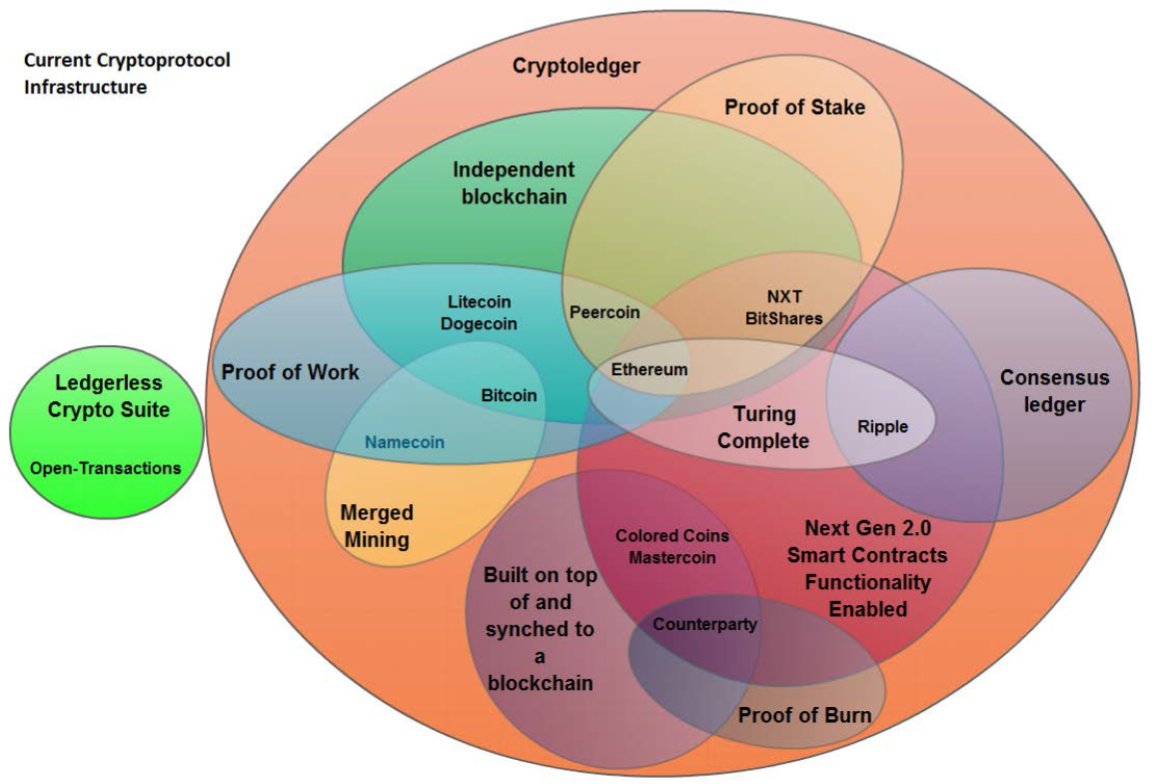
\includegraphics[width=0.85\columnwidth]{current_protocols.png}
        \captionsetup{labelformat=empty}
    \end{figure}
\end{frame}

\begin{frame}
    \frametitle{Методы, алгоритмы и технологии}
    \begin{multicols}{2}
        \begin{itemize}
            \item Сравнительный анализ алгоритмов и протоколов
            \item Язык Python 3.6
            \item {\LaTeX} (дистрибутив XeTeX) для презентаций и текста
        \end{itemize}
        \bigskip
        \columnbreak
        \begin{figure}
            
\includegraphics[width=\columnwidth]{gear.png}
            \captionsetup{labelformat=empty}
        \end{figure}
    \end{multicols}
\end{frame}

\begin{frame}
    \frametitle{Список используемых источников}
    % \nocite{*}
    % \printbibliography{}
    [1]: \textbf{Swanson, T.} (2014) \emph{Great Chain of Numbers a Guide to
    Smart Contracts, Smart Property and Trustless Asset Management}

    [2]: \textbf{Satoshi N.} (2007) \emph{Bitcoin: A Peer-to-Peer Electronic Cash System}

    [3]: \textbf{Aladin, D.} (2017) \emph{Blockchain Documentation}

    [4]: \textbf{Cryptocurrency} (2018)
    \emph{\small{https://en.wikipedia.org/wiki/Cryptocurrency}}

\end{frame}

\begin{frame}[c]
\begin{center}
\frametitle{\LARGE Спасибо за внимание!}

{\LARGE \inserttitle}

\bigskip

{\insertauthor}

\bigskip\bigskip

{\insertinstitute}

\bigskip\bigskip

{\large \insertdate}
\end{center}
\end{frame}

\end{document}


% EOF

